\documentclass[
	10pt,								% globale Schriftgröße
	parskip=half-,						% setzt Absatzabstand hoch
	paper=a4,							% Format
	english,ngerman,					% lädt Sprachpakete
	]{scrartcl}							% Dokumentenklasse

% //////////////////// Pakete laden ////////////////////
\usepackage{amsmath}			% MUSS vor fontspec geladen werden
\usepackage{mathtools}			% modifiziert amsmath
\usepackage{amssymb}			% mathematische symbole, für \ceckmarks
\usepackage{amsthm}				% für proof
\usepackage{mathrsfs}			% für \mathscr
\usepackage{latexsym}
\usepackage{marvosym}				% für Lightning

\usepackage{fontspec} 			% funktioniert nur mit den neueren Compilern z.B. XeLaTeX
\usepackage{microtype}			% für bessere Worttrennung
\usepackage[ngerman]{babel} 	% Spracheinstellung
\usepackage{lmodern}			% verändert verwendete Schriftart, damit sie weniger pixelig ist

\usepackage{verbatim}
\usepackage{listings}			% Für Quellcode

\usepackage{graphicx}
\usepackage{tabularx}			% für Tabellen mit gleicher Spaltenbreite und automatischen Umbrüchen
\usepackage{fullpage}
\usepackage{multirow}			% für multirow in tabulars
\usepackage{rotate}
\usepackage[cmyk,table]{xcolor} % um Farben zu benutzen, kann mehr als das Paket color
\usepackage[					% Verlinkungen
	colorlinks,					% farbige Schrift, statt farbiger Rahmen
	linktocpage,				% verlinkt im Abb.Verzeichnis Seitenzahl statt Bildunterschrift
	linkcolor=blue				% setzt Farbe der Links auf blau
	]{hyperref}					% nur für digitale Anwendungen, url = "http://www.example.com"
%\usepackage{url}				% für Webadressen wie e-mail usw.: "\url{http://www.example.com}"

\usepackage{enumerate}			% für versch. Aufzählungezeichen wie z.B. a)
\usepackage{xspace}				% folgt ein Leerzeichen nach einem \Befehl, wird es nicht verschluckt.
\usepackage{cancel}				% für das Durchstreichen u.a. in Matheformeln mit \cancel
\usepackage{float}              % zum Forcieren der Position von figure-Umgebungen
\usepackage{ifthen}				% neceassary for \forloop und \whiledo

% zum Zeichnen (u.a. von Graphen)
\usepackage{fp}
\usepackage{tikz}
\usetikzlibrary{tikzmark}			% für \tikzmark{toRemember}
\usetikzlibrary{positioning}	% verbesserte Positionierung der Knoten
\usetikzlibrary{automata}		% für Automaten (GTI)
\usetikzlibrary{arrows}
\usetikzlibrary{shapes}
\usetikzlibrary{decorations.pathmorphing}
\usetikzlibrary{decorations.pathreplacing}
\usetikzlibrary{decorations.shapes}
\usetikzlibrary{decorations.text}

% //////////////////// Syntaxhighlighting ////////////////////
\lstloadlanguages{Python, Haskell, [LaTeX]TeX, Java}
\lstset{
   basicstyle=\footnotesize\ttfamily,	% \scriptsize the size of the fonts that are used for the code
   backgroundcolor = \color{bgcolour},	% legt Farbe der Box fest
   breakatwhitespace=false,	% sets if automatic breaks should only happen at whitespace
   breaklines=true,			% sets automatic line breaking
   captionpos=t,				% sets the caption-position to bottom, t for top
   commentstyle=\color{codeblue}\ttfamily,% comment style
   frame=single,				% adds a frame around the code
   keepspaces=true,			% keeps spaces in text, useful for keeping indentation
							% of code (possibly needs columns=flexible)
   keywordstyle=\bfseries\ttfamily\color{codepurple},% keyword style
   numbers=left,				% where to put the line-numbers;
   							% possible values are (none, left, right)
   numberstyle=\tiny\color{codegreen},	% the style that is used for the line-numbers
   numbersep=5pt,			% how far the line-numbers are from the code
   stepnumber=1,				% nummeriert nur jede i-te Zeile
   showspaces=false,			% show spaces everywhere adding particular underscores;
							% it overrides 'showstringspaces'
   showstringspaces=false,	% underline spaces within strings only
   showtabs=false,			% show tabs within strings adding particular underscores
   flexiblecolumns=false,
   tabsize=1,				% the step between two line-numbers. If 1: each line will be numbered
   stringstyle=\color{orange}\ttfamily,	% string literal style
   numberblanklines=false,				% leere Zeilen werden nicht mitnummeriert
   xleftmargin=1.2em,					% Abstand zum linken Layoutrand
   xrightmargin=0.4em,					% Abstand zum rechten Layoutrand
   aboveskip=2ex, 
}

\lstdefinestyle{py}{
   language=Python,
}
\lstdefinestyle{hs}{
   language=Haskell,
}
\lstdefinestyle{tex}{
	language=[LaTeX]TeX,
	escapeinside={\%*}{*)},     % if you want to add LaTeX within your code
	texcsstyle=*\bfseries\color{blue},% hervorhebung der tex-Schlüsselwörter
	morekeywords={*,$,\{,\},\[,\],lstinputlisting,includegraphics,
	rowcolor,columncolor,listoffigures,lstlistoflistings,
	subsection,subsubsection,textcolor,tableofcontents,colorbox,
	fcolorbox,definecolor,cellcolor,url,linktocpage,subtitle,
	subject,maketitle,usetikzlibrary,node,path,addbibresource,
	printbibliography},% if you want to add more keywords to the set
     numbers=none,
     numbersep=0pt,
     xleftmargin=0.4em,
}

\lstdefinestyle{java}{
	language=Java,
	extendedchars=true,		% lets you use non-ASCII characters;
   						% for 8-bits encodings only, does not work with UTF-8
}

\lstdefinelanguage[x64]{Assembler}     % add a "x64" dialect of Assembler
   [x86masm]{Assembler} % based on the "x86masm" dialect
   % with these extra keywords:
   {morekeywords={CDQE,CQO,CMPSQ,CMPXCHG16B,JRCXZ,LODSQ,MOVSXD, %
                  POPFQ,PUSHFQ,SCASQ,STOSQ,IRETQ,RDTSCP,SWAPGS, %
                  rax,rdx,rcx,rbx,rsi,rdi,rsp,rbp, %
                  r8,r8d,r8w,r8b,r9,r9d,r9w,r9b}
}					% for 8-bits encodings only, does not work with UTF-8

\lstdefinestyle{c}{
	language=c,
	extendedchars=true,		% for 8-bits encodings only, does not work with UTF-8
}

% //////////////////// eigene Kommandos ////////////////////
\newcommand\FU{Freie Universität Berlin\xspace}% benötigt package xspace
\newcommand\gdw{g.\,d.\,w.\xspace}
\newcommand\oBdA{o.\,B.\,d.\,A.\xspace}
\newcommand{\Eu}{\texteuro}
\newcommand\N{\mathbb{N}\xspace}
\newcommand\Q{\mathbb{Q}\xspace}
\newcommand\R{\mathbb{R}\xspace}
\newcommand\Z{\mathbb{Z}\xspace}
\newcommand\ohneNull{\ensuremath{\backslash\lbrace 0\rbrace}}% \{0}
\let\dhALT\dh	% Schreibt Befehl \dh in \dhALT um
\renewcommand\dh{d.\,h.\xspace}	%renew überschreibt command \dh
\newcommand\Bolt{\;\text{\LARGE\raisebox{-0.3em}{\Lightning}\normalsize}\xspace}% Blitz
\newcommand\zz{\ensuremath{\raisebox{+0.25ex}{Z}% zu zeigen
			\kern-0.4em\raisebox{-0.25ex}{Z}%
			\;\xspace}}
\newcommand{\from}{\ensuremath{\colon}}
\newcommand{\floor}[1]{\lfloor{#1}\rfloor}
\newcommand{\ceil}[1]{\lceil{#1}\rceil}
 \renewcommand{\L}{\ensuremath{\mathcal{L}}\xspace}
 \renewcommand{\P}{\ensuremath{\mathcal{P}}\xspace}
 \newcommand{\NL}{\ensuremath{\mathcal{N}\kern-0.2em\mathcal{L}}\xspace}
 \newcommand{\NP}{\ensuremath{\mathcal{NP}}\xspace}

% //////////////////// Mathefunktionen ////////////////////
\DeclareMathOperator{\Landau}{\mathcal{O}}
\DeclareMathOperator{\True}{True}
\DeclareMathOperator{\False}{False}

% //////////////////// eigene Theoreme ////////////////////
\newtheorem{theorem}{Satz}
\newtheorem{corollary}[theorem]{Folgerung}
\newtheorem{lemma}[theorem]{Lemma}
\newtheorem{observation}[theorem]{Beobachtung}
\newtheorem{definition}[theorem]{Definition}
\newtheorem{Literatur}[theorem]{Literatur}
% konfiguriert proof
\makeatletter
\newenvironment{Proof}[1][\proofname]{\par
  \pushQED{\qed}%
  \normalfont \topsep6\p@\@plus6\p@\relax
  \trivlist
  \item[\hskip\labelsep
%         \itshape
        \bfseries
    #1\@addpunct{.}]\ignorespaces
}{%
  \popQED\endtrivlist\@endpefalse
}
\makeatother

% //////////////////// eigene Farben ////////////////////
\let\definecolor=\xdefinecolor
\definecolor{FUgreen}{RGB}{153,204,0}
\definecolor{FUblue}{RGB}{0,51,102}

\definecolor{middlegray}{rgb}{0.5,0.5,0.5}
\definecolor{lightgray}{rgb}{0.8,0.8,0.8}
\definecolor{orange}{rgb}{0.8,0.3,0.3}
\definecolor{azur}{rgb}{0,0.7,1}
\definecolor{yac}{rgb}{0.6,0.6,0.1}
\definecolor{Pink}{rgb}{1,0,0.6}

\definecolor{bgcolour}{rgb}{0.97,0.97,0.97}
\definecolor{codegreen}{rgb}{0,0.6,0}
\definecolor{codegray}{rgb}{0.35,0.35,0.35}
\definecolor{codepurple}{rgb}{0.58,0,0.82}
\definecolor{codeblue}{rgb}{0.4,0.5,1}

% //////////////////// eigene Settings ////////////////////

\textheight = 230mm		% Höhe des Satzspiegels / Layouts
\footskip = 10ex			% Abstand zw. Fußzeile und Grundlinie letzter Textzeile
\parindent 0pt			% verhindert Einrückung der 1. Zeile eines Absatzes
\setkomafont{sectioning}{\rmfamily\bfseries}% setzt Ü-Schriften in Serifen, {disposition}										
\newcommand{\dozent}{Wolfgang Mulzer, Katharina Klost}					% <-- Names des Dozenten eintragen
\newcommand{\tutor}{Tobias Gleißner}						% <-- Name eurer Tutoriun eintragen
\newcommand{\tutoriumNo}{02}				% <-- Nummer im KVV nachschauen
\newcommand{\ubungNo}{02}									% <-- Nummer des Übungszettels
\newcommand{\veranstaltung}{Algorithmen, Datenstrukturen und Datenabstraktion}	% <-- Name der Lehrveranstaltung eintragen
\newcommand{\semester}{Semester}						% <-- z.B. SoSo 17, WiSe 17/18
\newcommand{\studenten}{Nicolas Höcker, Michael Wernitz}			% <-- Hier eure Namen eintragen
\newcommand{\aufgNo}{3}	

\usepackage{amsmath}
\usepackage{mathtools}
\usepackage{letltxmacro}
\usepackage{graphicx}
\usepackage{listings}
\usepackage{color}
% /////////////////////// BEGIN DOKUMENT /////////////////////////
\begin{document}							
% ////////////// Notenspiegel und Logo //////////////
\vspace*{-15ex}							% rückt Logo an den oberen Seitenrand
\makebox[\dimexpr\textwidth+1cm][r]{		%rechtsbündig und geht rechts 1cm über Layout hinaus
	\begin{minipage}{0.5\linewidth}
	\newcounter{AufgNo}
	\setcounter{AufgNo}{\aufgNo}
	\stepcounter{AufgNo}					% AufgNo++
	\newcounter{zahl}
	\def\and{&\xspace}
	\renewcommand{\arraystretch}{1.3}\setlength{\tabcolsep}{1em}
	\begin{tabular}{*{\value{AufgNo}}{|c} |}
		\hline
		\setcounter{zahl}{1}
		\whiledo{\value{zahl} < \value{AufgNo}}{%\AufgNo 
			\thezahl\and\stepcounter{zahl}%
		} $\sum$ \\ \hline
		\setcounter{zahl}{1}
		\whiledo{\value{zahl} < \value{AufgNo}}{%\AufgNo 
			\and\stepcounter{zahl}%
		} \\ \hline
	\end{tabular}

	%\forloop{ct}{1}{\value{ct} < 5}{}
	\end{minipage}
	\hfill
	\begin{minipage}{0.5\linewidth}
	\hfill \ifnum\aufgNo<9%				blendet ab 9 Aufgaben das Logo aus
	
\includegraphics[width=0.8\textwidth]{src/fu_logo} % fügt FU-Logo ein
	\fi
	\end{minipage}
}
% ////////////// Daten //////////////
\begin{center}
{\large \dozent}\par
{\huge \veranstaltung, \semester}\par
{\large TutorIn: \tutor, Tutorium \tutoriumNo}\par
{\Large Übung \ubungNo}\par 
{\large \studenten}\par
\today
\end{center}
\vspace{-3ex}							% Abstand
\rule{\linewidth}{0.8pt}				% horizontale Linie

\section{ Dünnbesetzte Polynome \hfill}
{\itshape Die neu erstellte Abspeicherung von sogenannten dünn besetzten Polynomen erfolgt durch Tupelbildung mit folgendem Schema. }

\begin{equation}
	\begin{aligned}
		p(x) = a_nx^n + a_{n-1}x^{n-1} + \dots + a_1x + a_0 \notag\\
	\end{aligned} 
\end{equation}
		\text{wird abgespeichert als eine nach Grad des Polynoms absteigend geordnete Liste aus Tupeln mit folgender Bedingung: } \\
\begin{equation}
	\begin{aligned}
		p(x) = [(a_{n},n), \dots , (a_l,l)] \text{ ,wobei } a_i \neq 0 \text{, } 0 \leq i,l \leq n \notag \\ 
		\text{ und für k (Anzahl der Nullpolynome) gilt: } k=0 \\		
	\end{aligned}
\end{equation}		

\begin{itemize}
	\item \textbf{Addition}\\
		Für die Addition zweier $p(x),q(x)$ Polynome gilt: \\
		\begin{equation}
			\begin{aligned}
			 \forall (a_i,i)\in p(x), \forall(b_l,l)\in q(x)\text{ : } (a_i,i)+(b_l,l) = (a_i+b_l,i \vee l) \Leftrightarrow i=l \notag \\
			\end{aligned}
		\end{equation}
		\textbf{Beispiel:} \\		
		 
	\item \textbf{Multiplikation} \\
		Für die Multiplikation von zwei Polynomen $p(x),q(x)$ gilt: \\
		\begin{equation}
			\begin{aligned}
				\forall (a_i,i)\in p(x), \forall(b_l,l)\in q(x)\text{ : } (a_i,i)+(b_l,l) &= (a_i*b_l,i*l)\quad 0\leq i,l \leq deg(p(x),deg(q(x)))\notag \\
				\\
				\forall (a_i,i)\in p(x), \forall(b_l,l)\in q(x)\text{ : } (a_i,i)+(b_l,l) &= (a_i*b_l,i*l+1)\Leftrightarrow i=1 \vee l=1 \notag \\ 
				\\ 	
				\forall (a_i,i)\in p(x), \forall(b_l,l)\in q(x)\text{ : } (a_i,i)+(b_l,l) &= (a_i*b_l,i)\Leftrightarrow l=0 \quad 0\leq i \leq deg(p(x) \\
				\\
				\forall (a_i,i)\in p(x), \forall(b_l,l)\in q(x)\text{ : } (a_i,i)+(b_l,l) &= (a_i*b_l,l)\Leftrightarrow i=0 \quad 0\leq l \leq deg(q(x))) \\					
			\end{aligned}
		\end{equation}
	\item Polynomauflösung $p(x)$ an Stelle $x_0$ \\
		\begin{equation}
			\begin{aligned}
				\forall (a_i,i)\in p(x)\text{ : } \displaystyle \sum_{0\leq i \leq n}(a_i * x_0^i) \notag \\			
			\end{aligned}
		\end{equation}
		wobei zur Potenzierung der im Tutorium besprochene 	Algorithmus mit $ O(n*log_2(n))$ angewendet wird\\	
\end{itemize}

\newpage
 
\begin{itemize}
	\item \textbf{Effizienz der Algorithmen} 
		\begin{enumerate}
			\item Addition
				Mit dem Algorithmus zur Addition sind wir im Vergleich zu der in der Vorlesung vorgestelltem Darstellung mit k-0-Koeffizienten effizienter, da wir auf die Abspeicherung dieser verzichten, wodurch wir nur noch $(n-k)$ (n - Grad des Polynoms), anstatt n Additionen (wie in der Darstellung aus der Vorlesung) durchführen müssen. Damit unterlassen wir unnötige Additionsoperationen von k-0-Koeffizienten. 
			\item Multiplikation
 				Unsere Darstellung bewährt sich auch bei der Multiplikation von zwei Polynomen $p(x),q(x)$, da hier keine $(k*k^')$-0-Produkte vorkommen (wobei $k$ bzw. $k^'$ - Anzahl der 0-Koeffizienten in $p(x)$ bzw. $q(x)$), da nur mit Koeffizienten $a_i \neq 0$ mit $0 \leq i \leq n$ gerechnet wird.\\
				Somit ist auch hier unser Algorithmus zur gewählten Darstellung effizienter als der in der Vorlesung vorgestellte.
			\item Auswertung an $x_0$
				Die Auswertung eines Polynoms $p(x)$ an einer Stelle $x_0$ ist ebenso effizienter als der in der Vorlesung vorgestellte Algorithmus. Dabei können k-0-Produkte die durch Multiplikation eines 0-Koeffizienten und der i-ten Potenz von $x_0$ entstehen würden, sowie die k-Additionen (Anzahl der 0-Koeffizienten) weggelassen werden, was unseren Algorithmus effizienter gestaltet. 
		\end{enumerate}
		
		\item \textbf{Implementierung der oben vorgestellten Darstellung von Polynomen}
		\begin{enumerate}
		  \item Addition		
			\lstinputlisting[style=py,									
			firstnumber={1},										
			firstline={10},											
			lastline={38}]											
			{src/ALP3_1_final.py}
		  \newpage	
		  \item Multiplikation
			\lstinputlisting[style=py,									
			firstnumber={39},										
			firstline={51},											
			lastline={77}]											
			{src/ALP3_1_final.py}
		  \item Auswertung an $x_0$
		  	\lstinputlisting[style=py,									
			firstnumber={78},										
			firstline={91},											
			lastline={99}]											
			{src/ALP3_1_final.py}
		\end{enumerate}
\end{itemize}
\newpage
\section{Experimentelles Sortieren \hfill}
	\begin{enumerate}
		\item Bubblesort - worst-case Laufzeit: $O(n^2)$
			\lstset{language=Java, 
  					 basicstyle=\small, 
   					keywordstyle=\color{blue!80!black!100}, 
   					identifierstyle=, 
   					commentstyle=\color{green!50!black!100}, 
  					stringstyle=\ttfamily, 
 					breaklines=true, 
   					numbers=left, 
   					numberstyle=\small, 
   					frame=single, 
   					backgroundcolor=\color{blue!3} 
					}
					 
			\lstinputlisting[style =javal,
			firstnumber = {1},
			firstline={11},
			lastline={42}]
			{src/BubbleSort.java}
			
			\newpage			
		\item QuickSort - worst-case Laufzeit: $O(n^2)$
			\lstset{language=Java, 
  					 basicstyle=\small, 
   					keywordstyle=\color{blue!80!black!100}, 
   					identifierstyle=, 
   					commentstyle=\color{green!50!black!100}, 
  					stringstyle=\ttfamily, 
 					breaklines=true, 
   					numbers=left, 
   					numberstyle=\small, 
   					frame=single, 
   					backgroundcolor=\color{blue!3} 
					}
					 
			\lstinputlisting[style =javal,
			firstnumber = {1},
			firstline={12},
			lastline={64}]
			{src/QuickSort.java}	
		 \newpage
		 	\item MergeSort - worst-case Laufzeit: $O(n*log(n))$
				\lstset{language=Java, 
  					 basicstyle=\small, 
   					keywordstyle=\color{blue!80!black!100}, 
   					identifierstyle=, 
   					commentstyle=\color{green!50!black!100}, 
  					stringstyle=\ttfamily, 
 					breaklines=true, 
   					numbers=left, 
   					numberstyle=\small, 
   					frame=single, 
   					backgroundcolor=\color{blue!3} 
					}
					 
			\lstinputlisting[style =javal,
			firstnumber = {1},
			firstline={23},
			lastline={70}]
			{src/MergeSort.java}	
		
	\end{enumerate}
\newpage
	\begin{itemize}
		\item Grafische Darstellung \\
		\begin{center}
			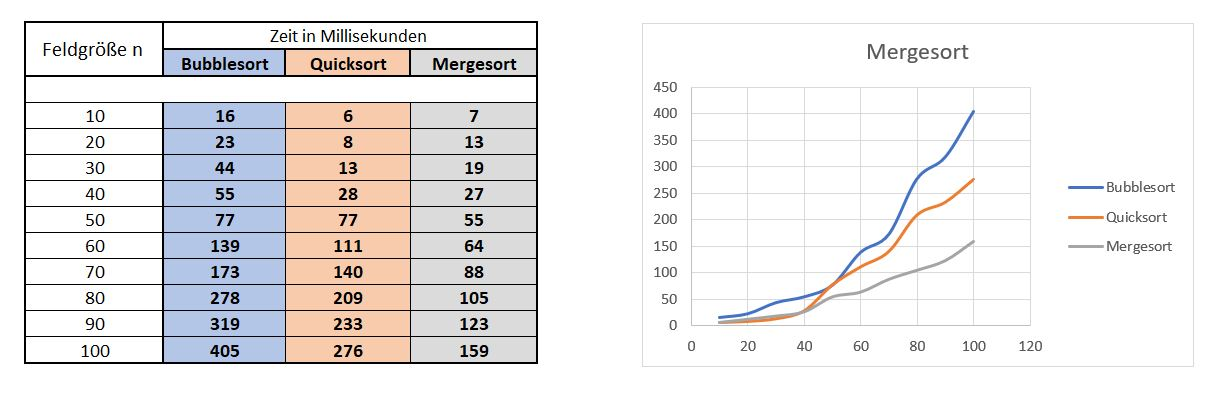
\includegraphics[width=1\textwidth]{src/Daten_Sortieralgorithmen.jpg}
		\end{center}
		\item Auswertung 
		Es ist deutlich zu erkennen, dass Bubblesort mit steigenden Eingabegrößen eine deutlich längere Ausführungszeit besitzt als Quicksort. Gleiches ist beim Vergleich von Quicksort und Mergesort festzustellen. Dieses Ergebnis spiegelt die den Sortieralgorithmen entsprechenden Komplexitätsklassen von Quick-/Bubblesort mit $O(n^2)$ und $O(n*log(n))$ von Mergesort. 
		\item Vorteile der Algorithmen
			\begin{enumerate}
				\item Bubblesort
					Bubblesort ist ein stabiler in-place Algorithmus der einfach zu implementieren und verstehen ist. Daher wird er meist für lehrreiche Zwecke verwendet, um z.B.: Komplexitäts- oder Korrektheitsbeweise durchzuführen.
				\item Quicksort
					Quicksort hat eine sehr hohe Ausführungsgeschwindigkeit, die durch eine kurze innere Schleife erreicht wird. Es ist ein in-place Verfahren, welches mit Ausnahme des benötigten Speicherplatzes für die Rekursionsaufrufe auf dem Aufruf-Stack keinen externen Speicherplatz benötigt. 
				\item Mergesort
				Mergesort ist ein sehr guter rekursiver Algorithmus, an dem das Divide and Conquer Prinzip sehr deutlich wird. Dieser Algorithmus hat eine Laufzeit von $O(n*log(n))$ sowohl im best-/average case als auch im worst case. Es ist zudem ein stabiles Verfahren. 
			\end{enumerate}
		\item Nachteile der Sortieralgorithmen
			\begin{enumerate}
				\item Bubblesort
					Bubblesort besitzen bei sehr großen n eine sehr schlechte Laufzeit, da er mehrmals durch die volle Liste iteriert und Element darin vergleicht. 			
				\item Quicksort
					Quicksort ist kein stabiles Verfahren, wodurch manche Datensätze falsch sortiert werden und es zu mehr oder weniger großen Komplikationen kommen kann. 
				\item Mergesort
					Mergesort benötigt zur Ausführung externen Speicher, da es kein in-place Algorithmus ist.  
			\end{enumerate}
		\item Verwendung der Algorithmen 
			Wenn nur mit sehr kleinen Eingaben gearbeitet wird und die Laufzeit nicht ins Gewicht fällt, ist Bubblesort eine einfache, schnell zu erstellende und stabile Lösung.
	Benötigt man eine hohe Ausführungsgeschwindigkeit und die Eingaben sind teils sortierte Listen ist Quicksort zu empfehlen. Dabei muss beachtet werden, dass Quicksort nicht satbil
		ist und die Eingabelisten nicht zu groß sein dürfen, da die Laufzeit gegen $O(n^2)$ geht.
	Mergesort ist unter den drei gewählten Verfahren das mit der besten Laufzeit in allen drei Fällen. Es ist aber nicht in-place, d.h. es wird zusätzlicher Speicher gebraucht, um Mergesort anzuwenden. Bei sehr großen Eingaben ist Mergesort unter den dreien sehr zu empfehlen, da es auch dort am schnellsten ist.
		\item Aussagen der O-Notation
	Schaut man sich die Laufzeitfunktion zu den gemessenen Eingaben an erkennt man, dass diese bei Bubblesort und Quicksort den Grad 2 besitzen, sie also quadratisch und damit in der Komplexitätsklasse 
		von $O(n^2)$ liegen, also die Funktion $f(n)=n^2$ die obere Grenze ist.
	Bei Mergesort lässt sich ähnliches erkennen. Dort stellt die Funktion $f(n)=n*log(n)$ die obere Grenze des Graphen der gemessenen Werte dar.

	\end{itemize}

\section{Türme von Hollywood}
 \begin{itemize}{a)}
 		\item 
 		Sei n die Anzahl der Scheiben und die drei vertikalen Stangen als A,B,C bezeichnet, wobei A die erste und C die letzte Stange ist. Um alle Scheiben 1 bis n von A nach C zu bewegen, müssen zuerst die größte Scheibe, also die Scheibe n, nach C bewegt werden. \\ Um dieses Problem zu lösen, müssen wir aber erst n-1 Scheiben nach B bewegt werden, um die Ordnungseigenschaft einzuhalten. Anschließend müssen die n-1 Scheiben nach C verschoben werden. \\
 		Dafür müssen wir aber, um n-1 Scheiben nach B zu bewegen, n-2 Scheiben nach C bewegen. Danach können wir die n-1-te Scheibe nach B bewegen, um anschließend die n-2 Scheiben von C nach b zu bewegen. \\
 		Wir zerlegen analog rekursiv weiter bis wir beim Problem angelangt sind, wohin wir Scheibe 1 bewegen. 
 		\begin{itemize}
 			\item Sei also n die eindeutige Scheibennummer für die Funktion $bewegeScheibe(n)$, so lautet die Anzahl von Verschiebungen: 
 			\begin{equation}
 				\begin{aligned}
 					bewegeScheibe(n) &= bewegeScheibe(n-1) + 1 + bewegeScheibe(n-1)\\
 					bewegeScheibe(1) &= 1 \notag\\
 				\end{aligned}
 			\end{equation}
 			\item wir können also vereinfachen zu: \\
 				\begin{equation}
 					\begin{aligned}
 						bewegeScheibe(n)= 1+ 2*bewegeScheibe(n-1) \notag\\
 					\end{aligned}
 				\end{equation}
 			\item Um pragmatisch die Anzahl der Scheiben für n=100 ermitteln zu können, müssen wir allerdings die geschlossene Formel für diese rekursive Funktion finden. 
 			
 			\item	
 			\begin{equation}
 				\begin{aligned}
 					b(n) &= 1 + 2*(b(n-1)) \\
 						 &= 1 + 2*(1+2*(b(n-2))) \\
 						 &= 1 + 2*(1+2*(1+2*(b(n-3)))) \\
 						 &= 1 + 2 + 4 + 8 * b(n-3) \\
 						 &= 1 +2^1 + 2^2 + 2^3 * b(n-1) \notag \\
 						 &= 1 + 2^1 + \dots + 2^{n-1}*b(n) \\
 						 &= 1 + 2^1 + \dots + 2^{n-1} \\
 						 &= \dots
 				\end{aligned}
 			\end{equation}
 			\item Beweis durch Induktion nach n \\
 			\begin{proof}
 				\begin{itemize}
 					\item I.A.: $n = 1$\\
 						\begin{equation}
 							\begin{aligned}
 								2^1-1 = 2-1 = 1 = b(1) \\
 								n=2 \\
 								b(2) &= b(1) + 1 + b(1) \\
 									 &= 1 + 2+1 \notag \\
 									 &= 3 \\
 								\\
 								2^2-1 = 3 = b(2)
 							\end{aligned}
 						\end{equation}
 					\item I.V.: $ b(n) = 2^n-1$ 
 					\item I.B.: $b(n+1) = 2^{n+1}-1$
 					\item I.S.: $ n \Rightarrow (n+1)$ \\
 						\begin{equation}
 							\begin{aligned}
 								b(n+1) &= 1 + 2*b(n) \\
 									   &\overset{IV}{=} 1 + 2(2^n-1) \\
 									   &=(2^n-1)+1+(2^n-1) \notag \\
 									   &= 2^{n+1}-1+1-1 \\
 									   &= 2^{n+1} -1 \\
 							\end{aligned}
 						\end{equation}					
 				\end{itemize}
 			\end{proof}
 			\item Also gilt für $n=100$:\\
 				\begin{equation}
 					\begin{aligned}
 						2^{100}-1 &= 1267650600228229401496703205375 \text{Tage} \\
 								  &\approx 3.473.015.343.091.039.456.155.351.248 \text{Jahre} \notag \\
 								  &\approx 3.473.015 \text{Trilliarden Jahre}
 					\end{aligned}
 				\end{equation}
 		\end{itemize}
 \end{itemize}

% /////////////////////// END DOKUMENT /////////////////////////
\end{document}

